% !TEX root = smc_bandits.tex
We empirically evaluate the proposed SMC-based Bayesian MAB framework
in non-stationary bandit scenarios
%\footnote{
%	Results in Appendix~\ref{assec:static_bandits_experiments_analytical}
%	validate the performance of SMC-based policies in stationary bandits.
%	We compare their performance to solutions based on analytically attainable posteriors
%	with Bernoulli and contextual linear Gaussian reward functions~\citep{ip-Kaufmann2012,ip-Garivier2011a,ic-Korda2013,ip-Agrawal2013a},
%	as well as for context-dependent binary rewards modeled with the logistic reward function~\cite{ic-Chapelle2011,j-Scott2015} ---Appendix~\ref{assec:static_bandits_experiments_logistic}.
%	Results showcase satisfactory performance across a wide range of stationary bandit parameterizations and sizes,
%	as SMC-based policies achieve the right exploration-exploitation tradeoff.
%}
with continuous, binary and discrete-categorical reward distributions.

Results in Appendix~\ref{assec:static_bandits_experiments_analytical}
validate the performance of SMC-based policies in stationary bandits.
We compare their performance to solutions based on analytically attainable posteriors
with Bernoulli and contextual linear Gaussian reward functions~\citep{ip-Kaufmann2012,ip-Garivier2011a,ic-Korda2013,ip-Agrawal2013a},
as well as for context-dependent binary rewards modeled with the logistic reward function~\cite{ic-Chapelle2011,j-Scott2015} ---Appendix~\ref{assec:static_bandits_experiments_logistic}.
Results showcase satisfactory performance across a wide range of stationary bandit parameterizations and sizes,
as SMC-based policies achieve the right exploration-exploitation tradeoff.

For results we present below, we simulate different parameterizations of dynamic linear models described in Section~\ref{ssec:linear_mixing_dynamics},
and present results for a variety of MAB environments with reward functions detailed in Sections~\ref{ssec:dynamic_bandits_gaussian},~\ref{ssec:dynamic_bandits_logistic} and~\ref{ssec:dynamic_bandits_categorical}.
Section~\ref{ssec:logged_data_bandits} illustrates
the ability of SMC-based bandit policies
to capture non-stationary trends in personalized news article recommendations.

The main evaluation metric is the cumulative regret of the bandit agent, as defined in Equation~\eqref{eq:mab_cumulative_regret},
with results averaged over 500 realizations.
We present results for SMC-based policies with $M=2000$ samples,
and provide an evaluation of the impact of $M$ in Appendix~\ref{asec:dynamic_bandits}.

\subsection{Non-stationary, linear Gaussian rewards}
\label{ssec:dynamic_bandits_gaussian}
% !TEX root = smc_bandits.tex
We simulate the following two-armed, contextual ($x_t\in\Real^2, \forall t$), linear Gaussian bandit:
\begin{equation}
\text{Scenario A}
\begin{cases}
	\vspace*{1ex}
	p(\theta_{t,a=0}|\theta_{t-1,a=0}): \\ \vspace*{1ex}
	\hspace*{10ex}\begin{pmatrix}
	\theta_{t,a=0,0}\\
	\theta_{t,a=0,1}\\
	\end{pmatrix} = \begin{pmatrix}
	0.9 & -0.1 \\
	-0.1 & 0.9 \\
	\end{pmatrix} \begin{pmatrix}
	\theta_{t-1,a=0,0}\\
	\theta_{t-1,a=0,1}\\
	\end{pmatrix} + \epsilon_{a=0} \;, \\ \vspace*{1ex}
	\hspace*{40ex} \text{where } \;  \epsilon_{a=0} \sim \N{\epsilon|0,0.01 \cdot\mathrm{I}},\\
	
	\vspace*{1ex}
	p(\theta_{t,a=1}|\theta_{t-1,a=1}): \\ \vspace*{1ex}
	\hspace*{10ex}\begin{pmatrix}
	\theta_{t,a=1,0}\\
	\theta_{t,a=1,1}\\
	\end{pmatrix} = \begin{pmatrix}
	0.9 & 0.1 \\
	0.1 & 0.9 \\
	\end{pmatrix} \begin{pmatrix}
	\theta_{t-1,a=1,0}\\
	\theta_{t-1,a=1,1}\\
	\end{pmatrix} + \epsilon_{a=1} \;, \\ \vspace*{1ex}
	\hspace*{40ex} \text{where } \;  \epsilon_{a=1} \sim \N{\epsilon|0,0.01 \cdot\mathrm{I}},\\
	
	p_a(Y|x,\theta_{t,a})=\N{Y|x^\top \theta_{t,a}, \sigma_a^2} \;.
\end{cases}
\label{eq:linear_mixing_dynamics_a}
\end{equation}

\begin{equation}
\text{Scenario B}
\begin{cases}
	\vspace*{1ex}
	p(\theta_{t,a=0}|\theta_{t-1,a=0}): \\ \vspace*{1ex}
	\hspace*{10ex}\begin{pmatrix}
	\theta_{t,a=0,0}\\
	\theta_{t,a=0,1}\\
	\end{pmatrix} = \begin{pmatrix}
	0.5 & 0.0 \\
	0.0 & 0.5 \\
	\end{pmatrix} \begin{pmatrix}
	\theta_{t-1,a=0,0}\\
	\theta_{t-1,a=0,1}\\
	\end{pmatrix} + \epsilon_{a=0} \;, \\ \vspace*{1ex}
	\hspace*{40ex} \text{where } \;  \epsilon_{a=0} \sim \N{\epsilon|0,0.01 \cdot\mathrm{I}},\\
	
	\vspace*{1ex}
	p(\theta_{t,a=1}|\theta_{t-1,a=1}): \\ \vspace*{1ex}
	\hspace*{10ex}\begin{pmatrix}
	\theta_{t,a=1,0}\\
	\theta_{t,a=1,1}\\
	\end{pmatrix} = \begin{pmatrix}
	0.9 & 0.1 \\
	0.1 & 0.9 \\
	\end{pmatrix} \begin{pmatrix}
	\theta_{t-1,a=1,0}\\
	\theta_{t-1,a=1,1}\\
	\end{pmatrix} + \epsilon_{a=1} \;, \\ \vspace*{1ex}
	\hspace*{40ex} \text{where } \;  \epsilon_{a=1} \sim \N{\epsilon|0,0.01 \cdot\mathrm{I}}, \\
	
	p_a(Y|x,\theta_{t,a})=\N{Y|x^\top \theta_{t,a}, \sigma_a^2} \;.
\end{cases}
\label{eq:linear_mixing_dynamics_b}
\end{equation}
 
The expected rewards driven by the dynamics of Equations~\eqref{eq:linear_mixing_dynamics_a} and~\eqref{eq:linear_mixing_dynamics_b} change over time,
inducing switches on the identity of the optimal arm.
%
For instance, for a given realization of Scenario A shown in Figure~\ref{fig:linear_mixing_dynamics_a_gaussian},
there is an optimal arm swap between time-instants $t=(300, 550)$, with arm 1 becoming the optimal for all $t\geq600$;
for a realization of Scenario B illustrated in Figure~\ref{fig:linear_mixing_dynamics_b_gaussian},
there is an optimal arm change around $t=100$, a swap around $t=600$,
with arm 1 becoming optimal again after $t\geq1600$.

Empirical results for SMC-based Bayesian policies in scenarios described by Equations~\eqref{eq:linear_mixing_dynamics_a} and~\eqref{eq:linear_mixing_dynamics_b}
are shown in Figures~\ref{fig:dynamic_bandits_linearGaussian_dknown} and \ref{fig:dynamic_bandits_linearGaussian_dunknown}.

% Linear Gaussian, known parameters
\begin{figure}[!h]
	\centering
	\begin{subfigure}[b]{0.45\textwidth}
		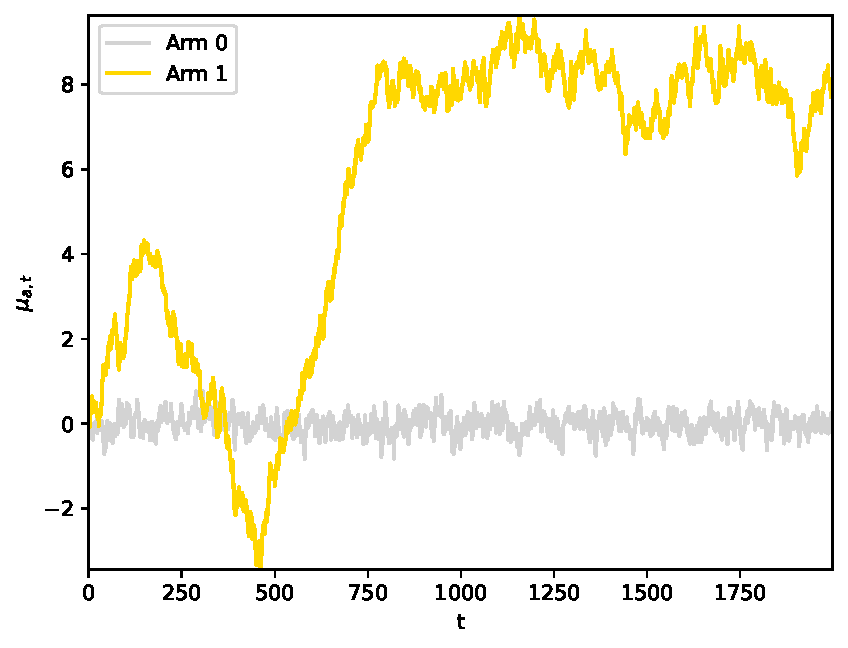
\includegraphics[width=\textwidth]{./fods_figs/dynamic/linearGaussian/dynamics_a}
		\caption{Expected per-arm rewards over time for Scenario A in Equation~\eqref{eq:linear_mixing_dynamics_a}.}
		\label{fig:linear_mixing_dynamics_a_gaussian}
	\end{subfigure}\qquad
	\begin{subfigure}[b]{0.45\textwidth}
		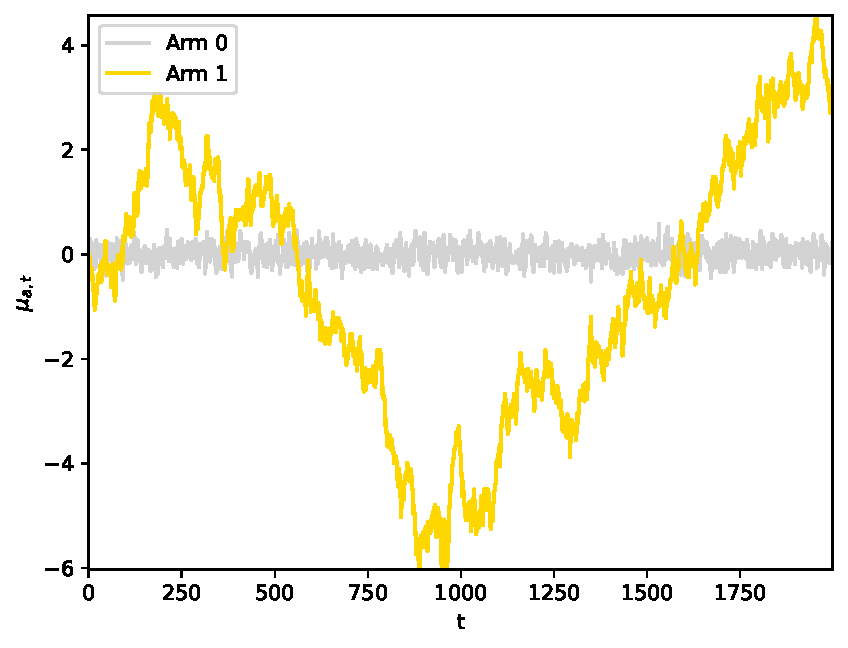
\includegraphics[width=\textwidth]{./fods_figs/dynamic/linearGaussian/dynamics_b}
		\caption{Expected per-arm rewards over time for Scenario B in Equation~\eqref{eq:linear_mixing_dynamics_a}.}
		\label{fig:linear_mixing_dynamics_b_gaussian}
	\end{subfigure}
	
	\begin{subfigure}[b]{0.47\textwidth}
		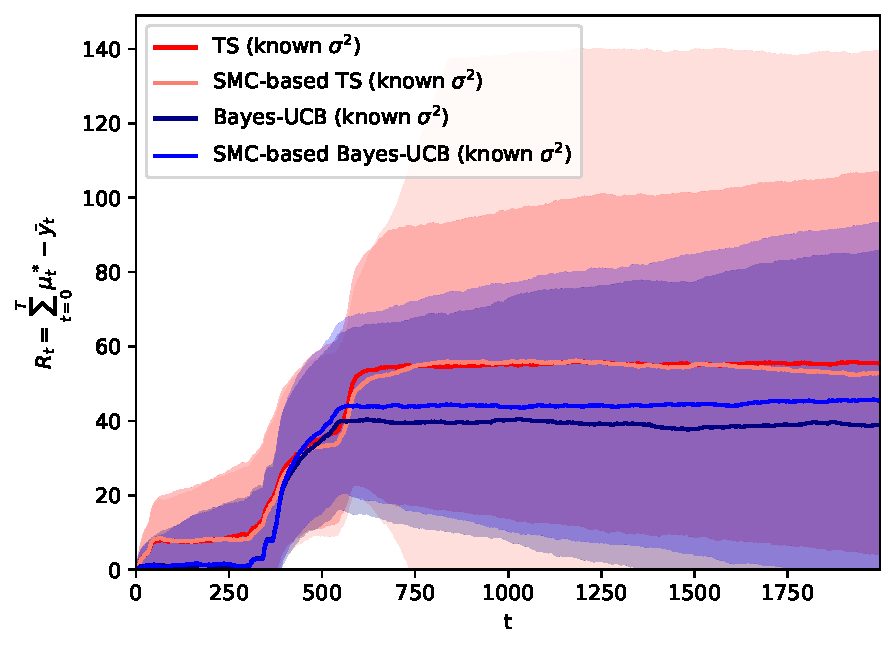
\includegraphics[width=\textwidth]{./fods_figs/dynamic/linearGaussian/a_M2000_cumulative_regret_dknown_knownsigma}
		\caption{Cumulative regret for SMC-based Bayesian policies in scenario A: known dynamic parameters.}
		\label{fig:dynamic_bandits_linearGaussian_a_cstatic_dknown_knownsigma}
	\end{subfigure}\qquad
	\begin{subfigure}[b]{0.47\textwidth}
		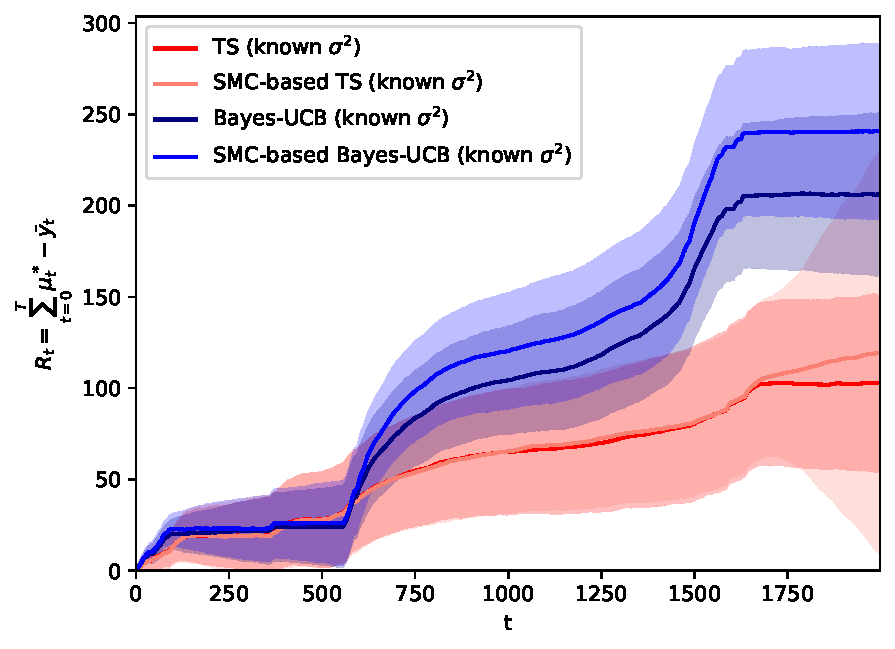
\includegraphics[width=\textwidth]{./fods_figs/dynamic/linearGaussian/b_M2000_cumulative_regret_dknown_knownsigma}
		\caption{Cumulative regret for SMC-based Bayesian policies in scenario B: known dynamic parameters.}
		\label{fig:dynamic_bandits_linearGaussian_b_cstatic_dknown_knownsigma}
	\end{subfigure}
	
	\caption{
		Mean regret (standard deviation shown as shaded region) in contextual, linear Gaussian bandit Scenarios A and B
		described in Equations~\eqref{eq:linear_mixing_dynamics_a}--\eqref{eq:linear_mixing_dynamics_b},
		when the bandit agent knows the latent dynamic parameterization.
		Notice how
		in Figures~\ref{fig:dynamic_bandits_linearGaussian_a_cstatic_dknown_knownsigma}--\ref{fig:dynamic_bandits_linearGaussian_b_cstatic_dknown_knownsigma}
		regret increases when the optimal arms swap
		(as shown in Figures~\ref{fig:linear_mixing_dynamics_a_gaussian}--\ref{fig:linear_mixing_dynamics_b_gaussian}).
		SMC-based policies successfully find the right exploration-exploitation tradeoff,
		with minimal additional regret incurred in comparison to their analytical alternatives. 
	}
	\label{fig:dynamic_bandits_linearGaussian_dknown}
\end{figure}

We study linear dynamics with Gaussian reward distributions with known parameters in Figure~\ref{fig:dynamic_bandits_linearGaussian_dknown},
of interest as it allows us to validate the SMC-based random measure in comparison to the optimal, closed-form posterior
---the Kalman filter~\cite{j-Kalman1960}---
under the assumption of known dynamic parameters.

We observe satisfactory cumulative regret performance in Figure~\ref{fig:dynamic_bandits_linearGaussian_dknown}:
\ie SMC-based Bayesian agents' cumulative regret is sublinear.
Policies that compute and use SMC random measure posteriors
incur in minimal regret loss 
in comparison to the optimal Kalman filter-based agent.
Namely, the shape of the regret curves of \textit{TS} and \textit{SMC-based TS}
(\textit{Bayes-UCB} and \textit{SMC based Bayes-UCB}, respectively) in Figure~\ref{fig:dynamic_bandits_linearGaussian_dknown} is equivalent,
with minimal differences in average cumulative regret when compared to the volatility across realizations.
Importantly, all policies are able to adapt to the changes over time of the identify of the optimal arm. 

We illustrate in Figure~\ref{fig:dynamic_bandits_linearGaussian_dunknown}
a more realistic scenario, where the dynamic parameterization is unknown to the bandit agent.

We observe in Figures~\ref{fig:dynamic_bandits_linearGaussian_a_cstatic_dknown_unknownsigma}--\ref{fig:dynamic_bandits_linearGaussian_b_cstatic_dknown_unknownsigma} that,
in the case of unknown reward variances ($\sigma_a^2, \forall a)$,
SMC-based policies perform comparably well.
In these cases,
the agents' reward model is not Gaussian,
but Student-t distributed, as per the marginalized posterior in Equation~\eqref{eq:t_posterior_mean}.
The regret loss associated with the uncertainty about $\sigma_a^2$ is minimal for SMC-based Bayesian agents,
and does not hinder the ability of the proposed SMC-based policies
to find the right exploration-exploitation balance:
\ie regret is sublinear, and the agents adapt to switches in the identity of the optimal arm.

We illustrate in Figures~\ref{fig:dynamic_bandits_linearGaussian_a_cstatic_dunknown}--\ref{fig:dynamic_bandits_linearGaussian_b_cstatic_dunknown}
the most realistic, yet challenging, non-stationary contextual Gaussian bandit case:
one where none of the parameters of the model are known.
In this case, the agent must sequentially learn both the underlying dynamics ($L_a,\Sigma_a; \forall a$)
and the conditional reward function's variance ($\sigma_a^2, \forall a)$,
in order to infer the posterior distribution over the latent, time-varying sufficient statistics of interest,
to enable informed sequential decision making.

Cumulative regret results in Figures~\ref{fig:dynamic_bandits_linearGaussian_a_cstatic_dunknown}--\ref{fig:dynamic_bandits_linearGaussian_b_cstatic_dunknown}
showcase a regret performance loss due to the need to learn all these unknown parameters.
We observe noticeable (almost linear) regret increases when the dynamics of the parameters swap the identity of the optimal arm.
However, SMC-based Thompson sampling and Bayes-UCB agents are able to learn the evolution of the dynamic latent parameters,
and the corresponding time-varying expected rewards,
with enough accuracy to attain good exploration-exploitation balance:
\ie sublinear regret curves indicate the agent identified and played the optimal arm repeatedly.
Figure~\ref{fig:dynamic_bandits_linearGaussian_a_cstatic_dunknown} is clear evidence of the SMC-based agents' ability to recover from linear to no-regret regimes.

\begin{figure}[!h]
	\centering
	\begin{subfigure}[b]{0.45\textwidth}
		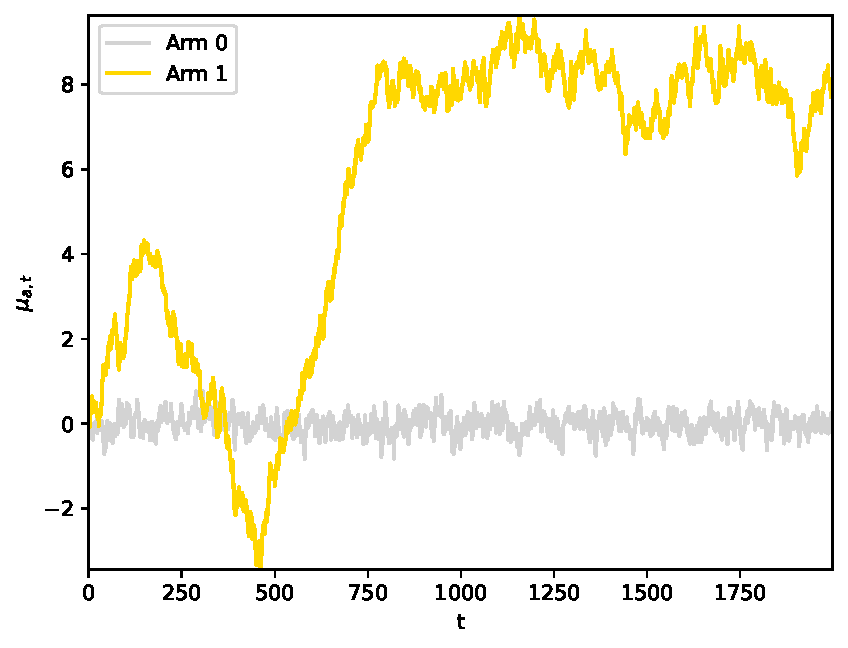
\includegraphics[width=\textwidth]{./fods_figs/dynamic/linearGaussian/dynamics_a}
		\caption{Expected per-arm rewards over time for Scenario A in Equation~\eqref{eq:linear_mixing_dynamics_a}.}
		\label{fig:linear_mixing_dynamics_a_gaussian_2}
	\end{subfigure}\qquad
	\begin{subfigure}[b]{0.45\textwidth}
		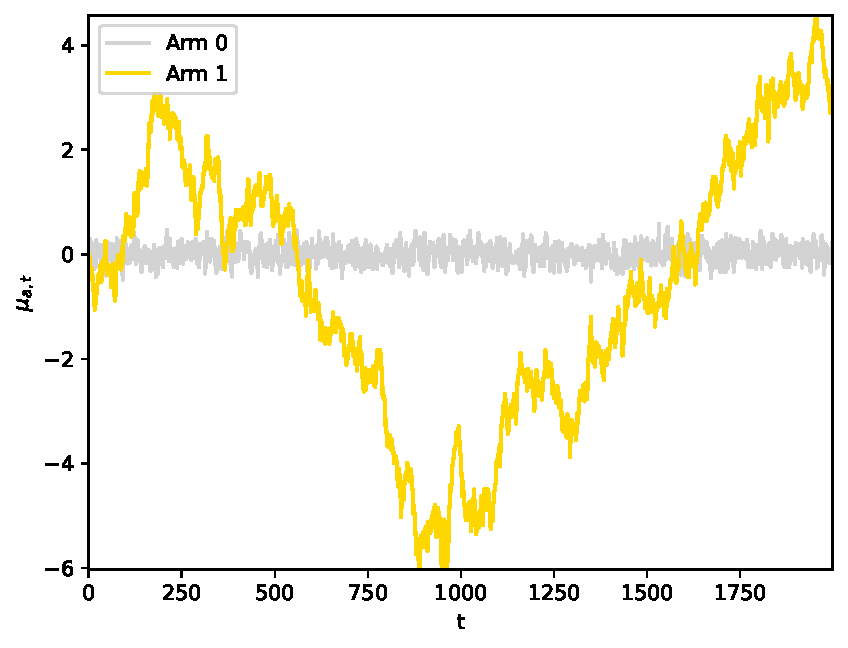
\includegraphics[width=\textwidth]{./fods_figs/dynamic/linearGaussian/dynamics_b}
		\caption{Expected per-arm rewards over time for Scenario B in Equation~\eqref{eq:linear_mixing_dynamics_a}.}
		\label{fig:linear_mixing_dynamics_b_gaussian_2}
	\end{subfigure}
	
	\begin{subfigure}[b]{0.47\textwidth}
		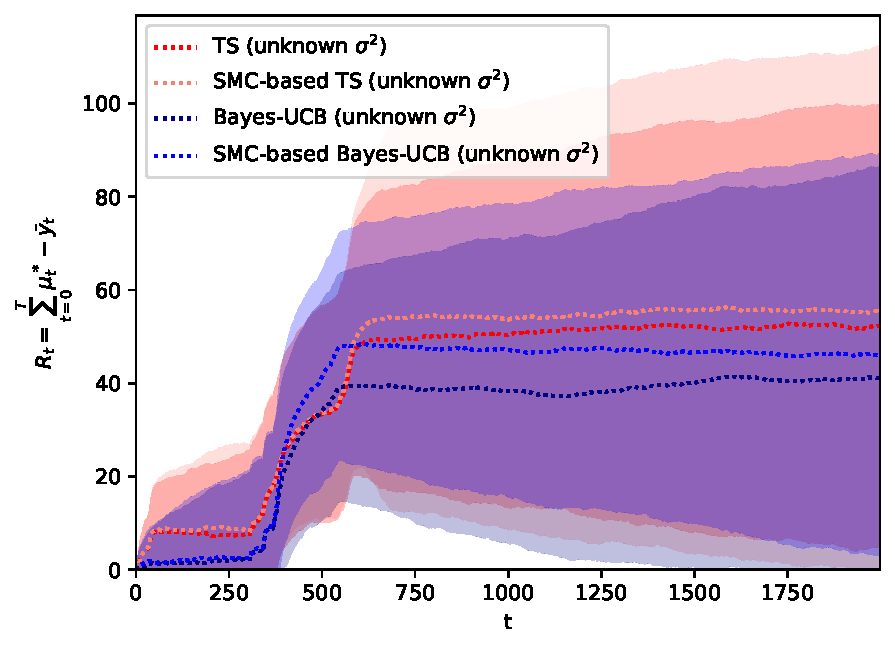
\includegraphics[width=\textwidth]{./fods_figs/dynamic/linearGaussian/a_M2000_cumulative_regret_dknown_unknownsigma}
		\caption{Cumulative regret for SMC-based Bayesian policies in scenario A: known dynamic parameters, unknown $\sigma_a, \forall a$.}
		\label{fig:dynamic_bandits_linearGaussian_a_cstatic_dknown_unknownsigma}
	\end{subfigure}\qquad
	\begin{subfigure}[b]{0.47\textwidth}
		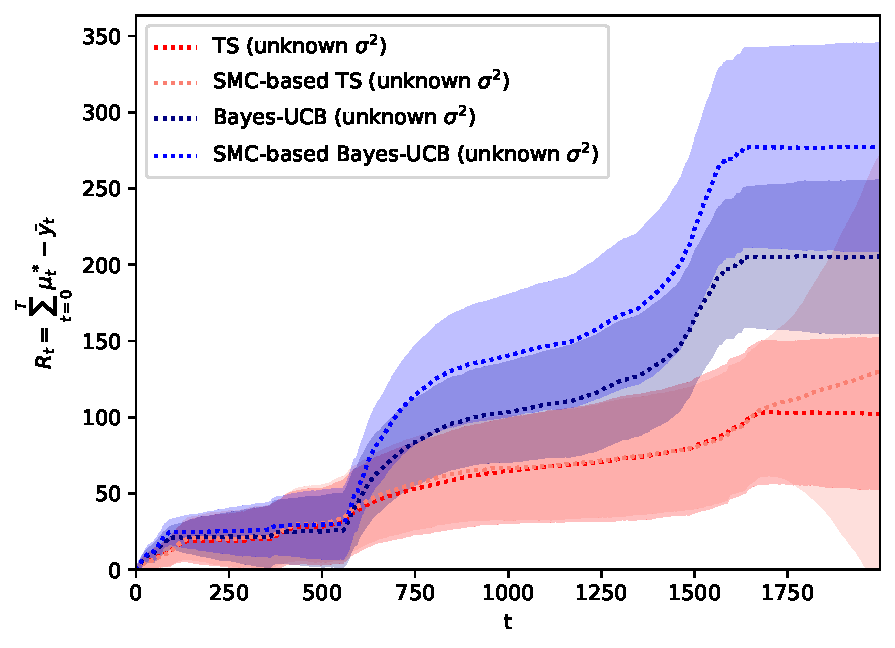
\includegraphics[width=\textwidth]{./fods_figs/dynamic/linearGaussian/b_M2000_cumulative_regret_dknown_unknownsigma}
		\caption{Cumulative regret for SMC-based Bayesian policies in scenario B: known dynamic parameters, unknown $\sigma_a, \forall a$.}
		\label{fig:dynamic_bandits_linearGaussian_b_cstatic_dknown_unknownsigma}
	\end{subfigure}
	
	\begin{subfigure}[b]{0.47\textwidth}
		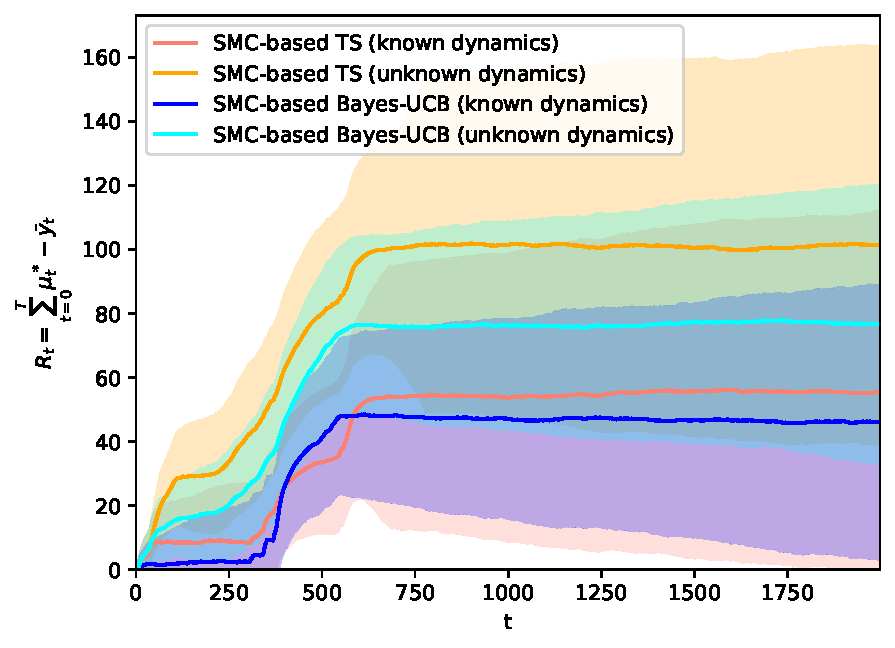
\includegraphics[width=\textwidth]{./fods_figs/dynamic/linearGaussian/a_M2000_cumulative_regret_dunknown}
		\caption{Cumulative regret for SMC-based Bayesian policies in scenario A: unknown dynamic parameters $L_a,\Sigma_a,\sigma_a^2, \forall a$.}
		\label{fig:dynamic_bandits_linearGaussian_a_cstatic_dunknown}
	\end{subfigure}\qquad
	\begin{subfigure}[b]{0.47\textwidth}
		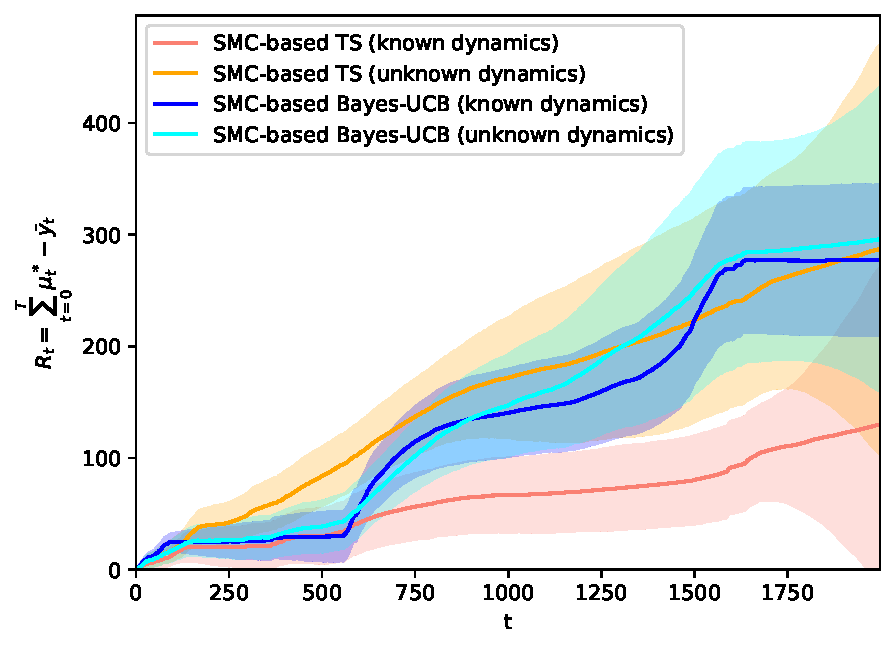
\includegraphics[width=\textwidth]{./fods_figs/dynamic/linearGaussian/b_M2000_cumulative_regret_dunknown}
		\caption{Cumulative regret for SMC-based Bayesian policies in scenario B: unknown dynamic parameters $L_a,\Sigma_a,\sigma_a^2, \forall a$.}
		\label{fig:dynamic_bandits_linearGaussian_b_cstatic_dunknown}
	\end{subfigure}
	\caption{
		Mean regret (standard deviation shown as shaded region) in contextual, linear Gaussian bandit Scenarios A and B
		described in Equations~\eqref{eq:linear_mixing_dynamics_a}--\eqref{eq:linear_mixing_dynamics_b},
		in the realistic setting of unknown dynamic parameters.
		Notice how
			in Figures~\ref{fig:dynamic_bandits_linearGaussian_a_cstatic_dknown_unknownsigma}--\ref{fig:dynamic_bandits_linearGaussian_b_cstatic_dunknown}
		the regret increases when the optimal arms swap
			(as shown in Figures~\ref{fig:linear_mixing_dynamics_a_gaussian_2}--\ref{fig:linear_mixing_dynamics_b_gaussian_2}).
		SMC-based policies find the right exploration-exploitation tradeoff even when the latent dynamic parameters are unknown.}
	\label{fig:dynamic_bandits_linearGaussian_dunknown}
\end{figure}


\clearpage
\subsection{Non-stationary, logistic rewards}
\label{ssec:dynamic_bandits_logistic}
% !TEX root = smc_bandits.tex
We here evaluate non-stationary, contextual, binary reward bandits.
We resort to the logistic reward function described in Equation~\eqref{eq:logistic_rewards},
with time-varying, latent parameter dynamics as described in the following scenarios:
\begin{equation}
\text{Scenario C}
\begin{cases}
\vspace*{1ex}
p(\theta_{t,a=0}|\theta_{t-1,a=0}): \\ \vspace*{1ex}
\hspace*{10ex}\begin{pmatrix}
\theta_{t,a=0,0}\\
\theta_{t,a=0,1}\\
\end{pmatrix} = \begin{pmatrix}
0.9 & -0.1 \\
-0.1 & 0.9 \\
\end{pmatrix} \begin{pmatrix}
\theta_{t-1,a=0,0}\\
\theta_{t-1,a=0,1}\\
\end{pmatrix} + \epsilon_{a=0} \;, \\ \vspace*{1ex}
\hspace*{40ex} \text{where } \;  \epsilon_{a=0} \sim \N{\epsilon|0,0.01 \cdot\mathrm{I}},\\

\vspace*{1ex}
p(\theta_{t,a=1}|\theta_{t-1,a=1}): \\ \vspace*{1ex}
\hspace*{10ex}\begin{pmatrix}
\theta_{t,a=1,0}\\
\theta_{t,a=1,1}\\
\end{pmatrix} = \begin{pmatrix}
0.9 & 0.1 \\
0.1 & 0.9 \\
\end{pmatrix} \begin{pmatrix}
\theta_{t-1,a=1,0}\\
\theta_{t-1,a=1,1}\\
\end{pmatrix} + \epsilon_{a=1}  \;, \\ \vspace*{1ex}
\hspace*{40ex} \text{where } \;  \epsilon_{a=1} \sim \N{\epsilon|0,0.01 \cdot\mathrm{I}},\\

p_a(Y|x,\theta_{t,a})=\frac{e^{y\cdot(x^\top\theta_{t,a}) }}{1+e^{(x^\top\theta_{t,a})}} \; .
\end{cases}
\label{eq:linear_mixing_dynamics_c}
\end{equation}

\begin{equation}
\text{Scenario D}
\begin{cases}
\vspace*{1ex}
p(\theta_{t,a=0}|\theta_{t-1,a=0}): \\ \vspace*{1ex}
\hspace*{10ex}\begin{pmatrix}
\theta_{t,a=0,0}\\
\theta_{t,a=0,1}\\
\end{pmatrix} = \begin{pmatrix}
0.5 & 0.0 \\
0.0 & 0.5 \\
\end{pmatrix} \begin{pmatrix}
\theta_{t-1,a=0,0}\\
\theta_{t-1,a=0,1}\\
\end{pmatrix} + \epsilon_{a=0}  \;, \\ \vspace*{1ex}
\hspace*{40ex} \text{where } \;  \epsilon_{a=0} \sim \N{\epsilon|0,0.01 \cdot\mathrm{I}},\\

\vspace*{1ex}
p(\theta_{t,a=1}|\theta_{t-1,a=1}): \\ \vspace*{1ex}
\hspace*{10ex}\begin{pmatrix}
\theta_{t,a=1,0}\\
\theta_{t,a=1,1}\\
\end{pmatrix} = \begin{pmatrix}
0.9 & 0.1 \\
0.1 & 0.9 \\
\end{pmatrix} \begin{pmatrix}
\theta_{t-1,a=1,0}\\
\theta_{t-1,a=1,1}\\
\end{pmatrix} + \epsilon_{a=1}  \;, \\ \vspace*{1ex}
\hspace*{40ex} \text{where } \;  \epsilon_{a=1} \sim \N{\epsilon|0,0.01 \cdot\mathrm{I}}, \\

p_a(Y|x,\theta_{t,a})=\frac{e^{y\cdot(x^\top\theta_{t,a}) }}{1+e^{(x^\top\theta_{t,a})}} \; .
\end{cases}
\label{eq:linear_mixing_dynamics_d}
\end{equation}

For bandits with logistic rewards,
there are no closed form posteriors;
hence, one needs to resort to approximations,
\eg a Laplace approximation as in~\citep{ic-Chapelle2011} for the stationary case.
However, there are no bandit algorithms for the non-stationary logistic scenarios described above.
%
On the contrary, SMC-based Bayesian policies can easily accommodate this setting,
by updating posterior random measures $p_M(\theta_{t}|\HH_{1:t})$ as in Algorithm~\ref{alg:sir-mab},
for both stationary (evaluated in Appendix~\ref{assec:static_bandits_experiments_logistic}) and non-stationary bandits we report here.

Figure~\ref{fig:dynamic_bandits_logistic} illustrates how
SMC-based Bayesian policies adapt to non-stationary optimal arm switches under contextual, binary reward observations,
achieving sublinear regret.
Results in Figures~\ref{fig:linear_mixing_dynamics_d_logistic}--\ref{fig:dynamic_bandits_d_logistic_cstatic}
also showcase how a bandit agent's regret suffers when learning unknown parameters of the latent dynamics.
%
Even though this is a particularly challenging problem,
presented evidence suggests that
SMC-based policies do learn the underlying latent dynamics from contextual binary rewards.

Notably, proposed policies are able to successfully identify which arm to play:
\ie both \textit{SMC-based TS and SMC-based UCB} ---with no dynamic parameter knowledge---
are able to flatten their regret
for $t\geq 650$ in Figure~\ref{fig:dynamic_bandits_c_logistic_cstatic} and
$t\geq 1750$ in Figure~\ref{fig:dynamic_bandits_d_logistic_cstatic}.

% Logistic results 
\begin{figure}[!h]
	\begin{subfigure}[b]{0.45\textwidth}
		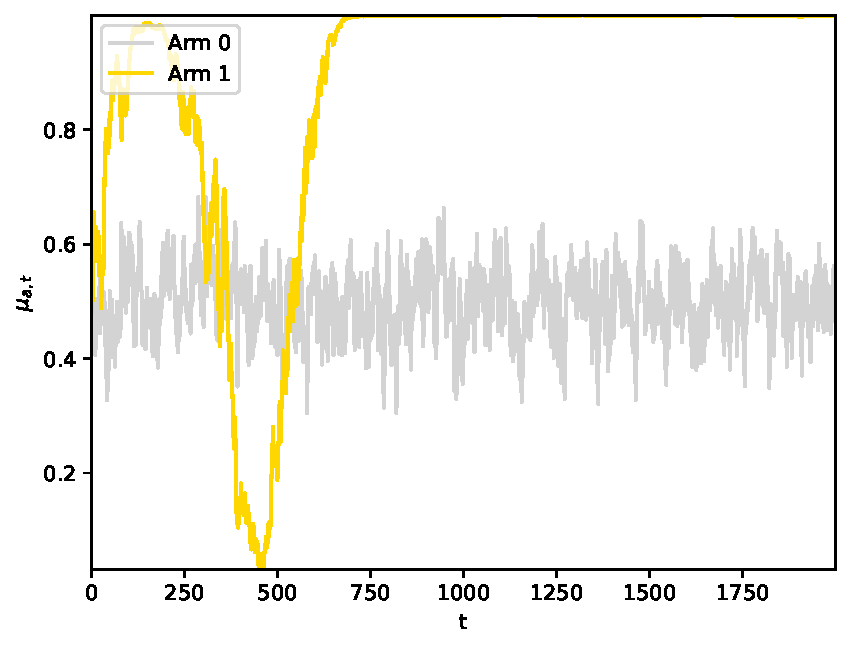
\includegraphics[width=\textwidth]{./fods_figs/dynamic/logistic/dynamics_c}
		\caption{Expected per-arm rewards over time for Scenario C in Equation~\eqref{eq:linear_mixing_dynamics_c}.
			Notice the early optimal arm change at $t\approx600$.
		}
		\label{fig:linear_mixing_dynamics_c_logistic}
	\end{subfigure}\qquad
	\begin{subfigure}[b]{0.45\textwidth}
		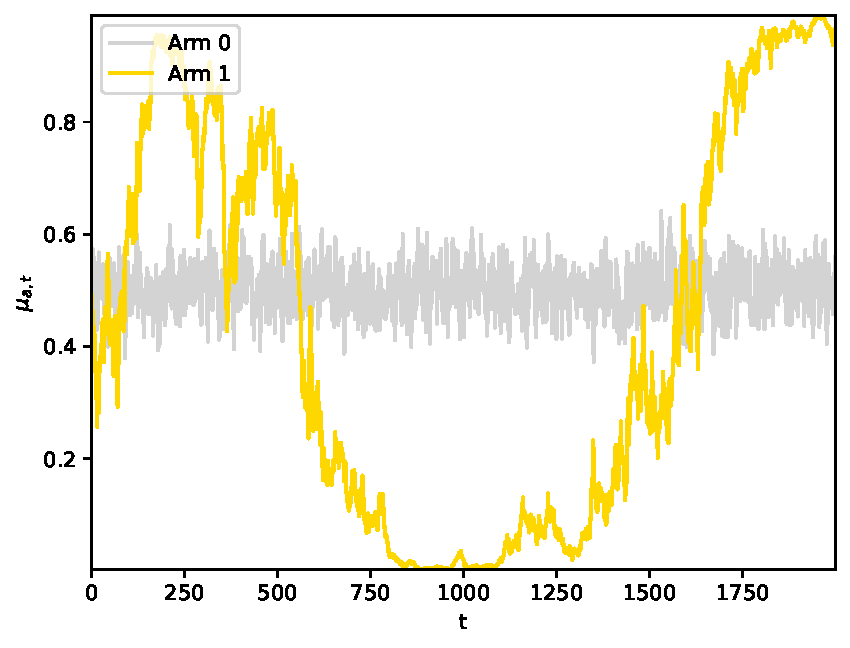
\includegraphics[width=\textwidth]{./fods_figs/dynamic/logistic/dynamics_d}
		\caption{Expected per-arm rewards over time for Scenario D in Equation~\eqref{eq:linear_mixing_dynamics_d}.
			Notice the late optimal arm change at $t\approx1650$.
		}
		\label{fig:linear_mixing_dynamics_d_logistic}
	\end{subfigure}
	
	\begin{subfigure}[b]{0.47\textwidth}
		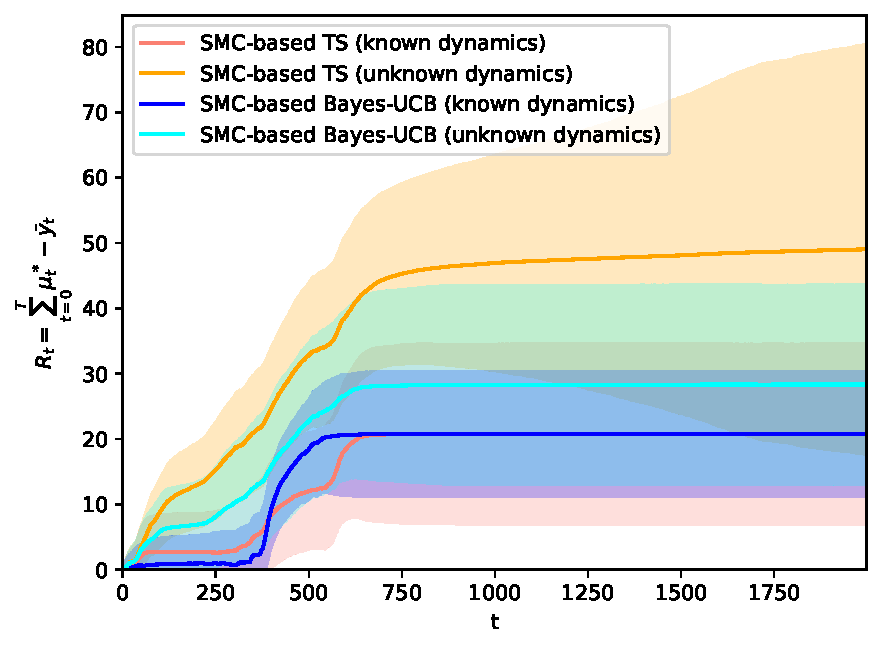
\includegraphics[width=\textwidth]{./fods_figs/dynamic/logistic/c_M2000_cumulative_regret_dunknown}
		\caption{Cumulative regret for SMC-based Bayesian policies in scenario C: known and unknown dynamic parameters.}
		\label{fig:dynamic_bandits_c_logistic_cstatic}
	\end{subfigure}\qquad
	\begin{subfigure}[b]{0.47\textwidth}
		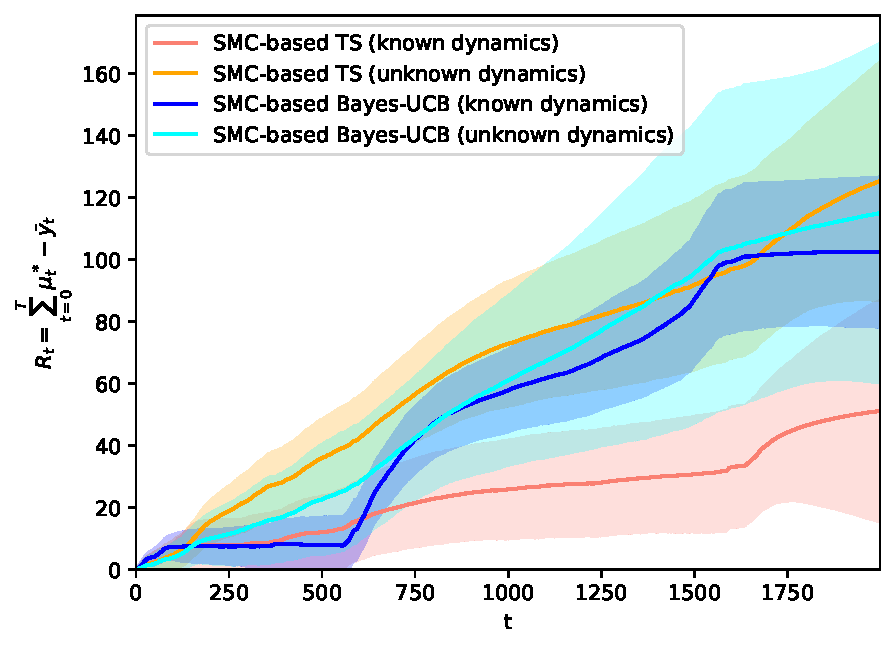
\includegraphics[width=\textwidth]{./fods_figs/dynamic/logistic/d_M2000_cumulative_regret_dunknown}
		\caption{Cumulative regret for SMC-based Bayesian policies in scenario D: known and unknown dynamic parameters.}
		\label{fig:dynamic_bandits_d_logistic_cstatic}
	\end{subfigure}
	\caption{
		Mean regret (standard deviation shown as shaded region) in contextual linear logistic dynamic bandit Scenarios C and D
		described in Equations~\eqref{eq:linear_mixing_dynamics_c}--\eqref{eq:linear_mixing_dynamics_d}.
		Notice the difference in early ($t\approx600$ in Scenario C) and late ($t\approx1650$ in Scenario D) optimal arm changes,
			as illustrated in Figures~\ref{fig:linear_mixing_dynamics_c_logistic}--\ref{fig:linear_mixing_dynamics_d_logistic},
		and their impact in regret,
			as showcased in Figures~\ref{fig:dynamic_bandits_c_logistic_cstatic}--\ref{fig:dynamic_bandits_d_logistic_cstatic}.
		SMC-based Bayesian policies adapt and find the right exploration-exploitation tradeoff.}
	\label{fig:dynamic_bandits_logistic}
\end{figure}


\clearpage
\subsection{Non-stationary, categorical rewards}
\label{ssec:dynamic_bandits_categorical}
% !TEX root = smc_bandits.tex
We evaluate SMC-based Bayesian policies in a bandit setting that remains elusive to state-of-the-art bandit algorithms:
non-stationary bandits with discrete-categorical, contextual rewards.
%
We simulate the following two- and three-armed categorical bandit scenarios,
where numerical rewards $Y=c$, for $c\in\{0,1,2\}$,
depend on a two-dimensional context $x_t\in\Real^2$,
with time-varying parameters $\theta_{a,c,t}$
obeying the following dynamics:

\begin{equation}
\text{Scenario E}
\begin{cases}
\vspace*{1ex}
p(\theta_{t,a=0,c}|\theta_{t-1,a=0,c})\;, \; \forall c \in \{0,1,2\}:\\ \vspace*{1ex}
\hspace*{10ex}\begin{pmatrix}
\theta_{t,a=0,c,0}\\
\theta_{t,a=0,c,1}\\
\end{pmatrix} = \begin{pmatrix}
0.9 & -0.1 \\
-0.1 & 0.9 \\
\end{pmatrix} \begin{pmatrix}
\theta_{t-1,a=0,c,0}\\
\theta_{t-1,a=0,c,1}\\
\end{pmatrix} + \epsilon_{a=0,c} \;, \\ \vspace*{1ex}
\hspace*{38ex} \text{where } \; \epsilon_{a=0,c} \sim \N{\epsilon|0,0.01 \cdot\mathrm{I}}, \\

\vspace*{1ex}
p(\theta_{t,a=1,c}|\theta_{t-1,a=1,c})\;, \; \forall c \in \{0,1,2\}:\\ \vspace*{1ex}
\hspace*{10ex}\begin{pmatrix}
\theta_{t,a=1,c,0}\\
\theta_{t,a=1,c,1}\\
\end{pmatrix} = \begin{pmatrix}
0.9 & 0.1 \\
0.1 & 0.9 \\
\end{pmatrix} \begin{pmatrix}
\theta_{t-1,a=1,c,0}\\
\theta_{t-1,a=1,c,1}\\
\end{pmatrix} + \epsilon_{a=1,c} \;, \\ \vspace*{1ex}
\hspace*{38ex} \text{where } \;  \epsilon_{a=1,c} \sim \N{\epsilon|0,0.01 \cdot\mathrm{I}},\\

p_a(Y=c|x,\theta_{t,a})=\frac{e^{(x^\top\theta_{t,a,c})}}{\sum_{c'=1}^C e^{(x^\top\theta_{t,a,c'})} } \; .
\end{cases}
\label{eq:linear_mixing_dynamics_e}
\end{equation}

\begin{equation}
\text{Scenario F}
\begin{cases}
\vspace*{1ex}
p(\theta_{t,a=0,c}|\theta_{t-1,a=0,c}) \;, \; \forall c \in \{0,1,2\}:\\ \vspace*{1ex}
\hspace*{10ex}\begin{pmatrix}
\theta_{t,a=0,c,0}\\
\theta_{t,a=0,c,1}\\
\end{pmatrix} = \begin{pmatrix}
0.9 & -0.1 \\
-0.1 & 0.9 \\
\end{pmatrix} \begin{pmatrix}
\theta_{t-1,a=0,c,0}\\
\theta_{t-1,a=0,c,1}\\
\end{pmatrix} + \epsilon_{a=0,c} \;, \\ \vspace*{1ex}
\hspace*{38ex} \text{where } \; \epsilon_{a=0,c} \sim \N{\epsilon|0,0.01 \cdot\mathrm{I}}, \\

\vspace*{1ex}
p(\theta_{t,a=1,c}|\theta_{t-1,a=1,c})\;, \; \forall c \in \{0,1,2\}:\\ \vspace*{1ex}
\hspace*{10ex}\begin{pmatrix}
\theta_{t,a=1,c,0}\\
\theta_{t,a=1,c,1}\\
\end{pmatrix} = \begin{pmatrix}
0.9 & 0.1 \\
0.1 & 0.9 \\
\end{pmatrix} \begin{pmatrix}
\theta_{t-1,a=1,c,0}\\
\theta_{t-1,a=1,c,1}\\
\end{pmatrix} + \epsilon_{a=1,c} \;, \\ \vspace*{1ex}
\hspace*{38ex} \text{where } \; \epsilon_{a=1,c} \sim \N{\epsilon|0,0.01 \cdot\mathrm{I}},\\

\vspace*{1ex}
p(\theta_{t,a=2,c}|\theta_{t-1,a=2,c})\;, \; \forall c \in \{0,1,2\}:\\ \vspace*{1ex}
\hspace*{10ex}\begin{pmatrix}
\theta_{t,a=2,c,0}\\
\theta_{t,a=2,c,1}\\
\end{pmatrix} = \begin{pmatrix}
0.9 & 0.1 \\
0.1 & 0.9 \\
\end{pmatrix} \begin{pmatrix}
\theta_{t-1,a=2,c,0}\\
\theta_{t-1,a=2,c,1}\\
\end{pmatrix} + \epsilon_{a=2,c} \;, \\ \vspace*{1ex}
\hspace*{38ex} \text{where } \; \epsilon_{a=2,c} \sim \N{\epsilon|0,0.01 \cdot\mathrm{I}},\\

p_a(Y=c|x,\theta_{t,a})=\frac{e^{(x^\top\theta_{t,a,c})}}{\sum_{c'=1}^C e^{(x^\top\theta_{t,a,c'})} } \; .
\end{cases}
\label{eq:linear_mixing_dynamics_f}
\end{equation}

These bandit scenarios accommodate a diverse set of expected reward dynamics,
for each realization of the noise processes $\epsilon_{a,c}, \forall a,c$,
and depending on the initialization of parameters $\theta_{0,a}$.
%
We illustrate per-arm, expected reward time-evolution for a realization
of the two-armed bandit Scenario E in Figure~\ref{fig:linear_mixing_dynamics_e_softmax},
and for the three-armed bandit Scenario F in Figure~\ref{fig:linear_mixing_dynamics_f_softmax}.

In all cases, expected rewards of each arm vary over time,
resulting in transient and recurrent swaps of the optimal arm's identity.
We show the corresponding cumulative regret of SMC-based Bayesian policies
in Figure~\ref{fig:dynamic_bandits_e_softmax_cstatic} for Scenario E,
and in Figure~\ref{fig:dynamic_bandits_f_softmax_cstatic} for Scenario F.

\begin{figure}[!ht]
	\centering
	\begin{subfigure}[b]{0.47\textwidth}
		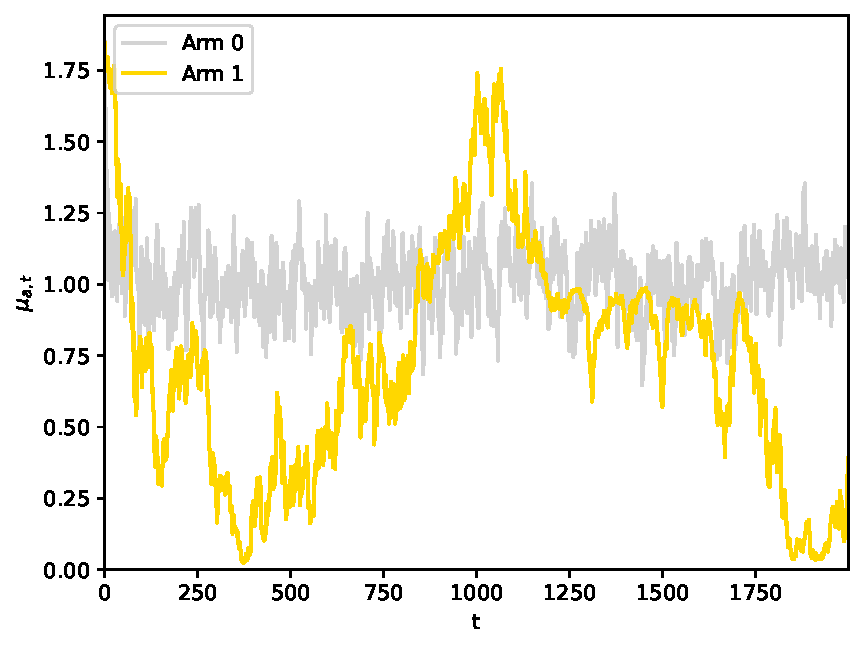
\includegraphics[width=\textwidth]{./fods_figs/dynamic/softmax/dynamics_e}
		\caption{Expected per-arm rewards over time for Scenario E in Equation~\eqref{eq:linear_mixing_dynamics_e}.
			Notice the optimal arm changes around $t\approx1000$.}
		\label{fig:linear_mixing_dynamics_e_softmax}%
	\end{subfigure}\qquad
	\begin{subfigure}[b]{0.47\textwidth}
		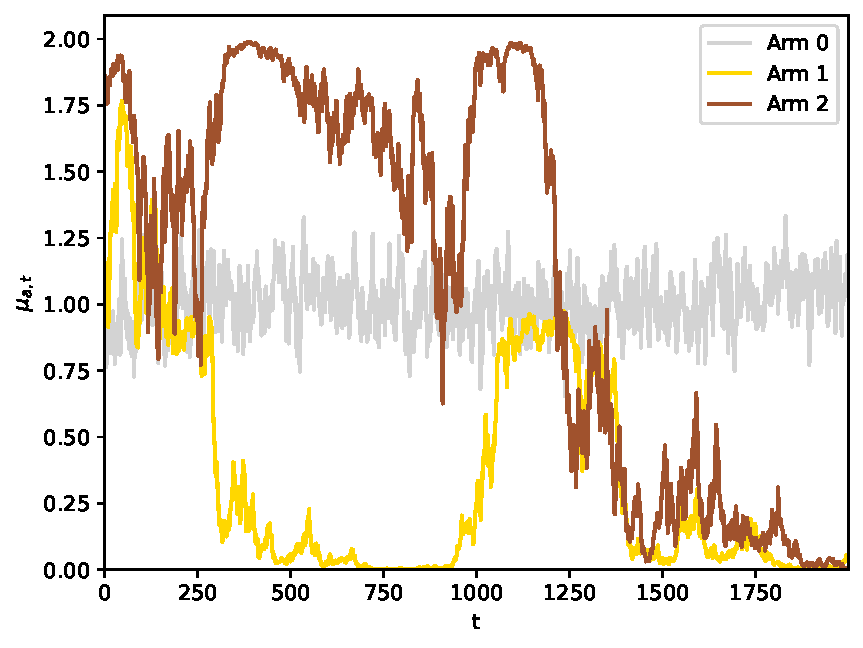
\includegraphics[width=\textwidth]{./fods_figs/dynamic/softmax/dynamics_f}
		\caption{Expected per-arm rewards over time for Scenario F in Equation~\eqref{eq:linear_mixing_dynamics_e}.
			Notice the optimal arm change around $t\approx1250$.}
		\label{fig:linear_mixing_dynamics_f_softmax}
	\end{subfigure} %
	
	\begin{subfigure}[b]{0.47\textwidth}
		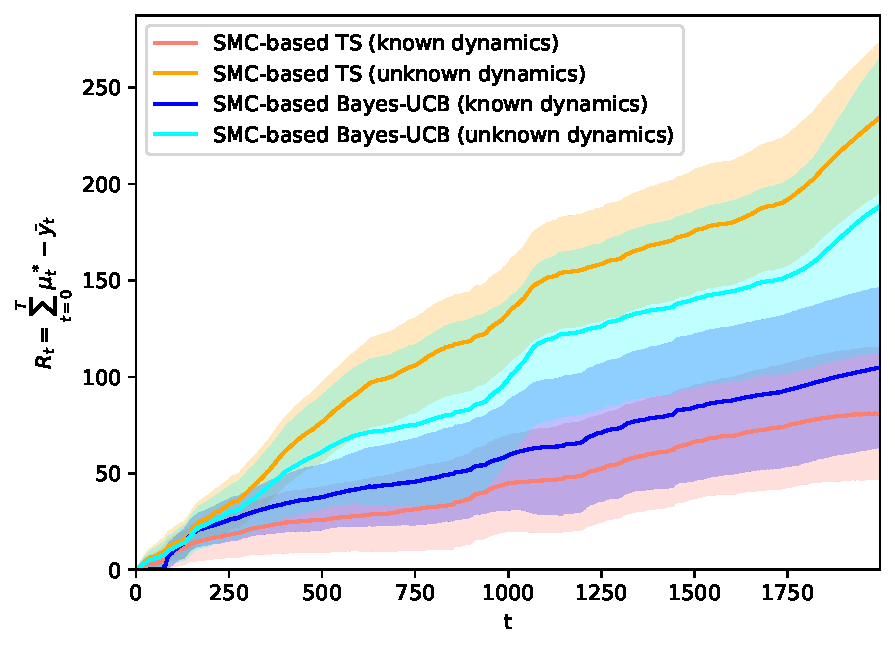
\includegraphics[width=\textwidth]{./fods_figs/dynamic/softmax/e_M2000_cumulative_regret_dunknown}
		\caption{Cumulative regret for SMC-based Bayesian policies in scenario E: known and unknown dynamic parameters.}
		\label{fig:dynamic_bandits_e_softmax_cstatic}%
	\end{subfigure}\qquad
	\begin{subfigure}[b]{0.47\textwidth}
		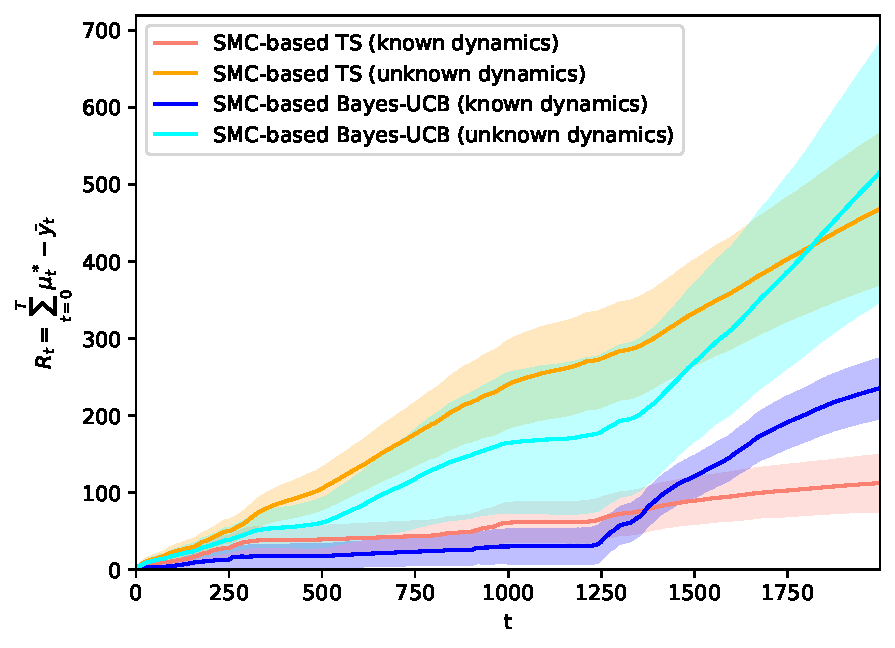
\includegraphics[width=\textwidth]{./fods_figs/dynamic/softmax/f_M2000_cumulative_regret_dunknown}
		\caption{Cumulative regret for SMC-based Bayesian policies in scenario F: known and unknown dynamic parameters.}
		\label{fig:dynamic_bandits_f_softmax_cstatic}%
	\end{subfigure}
	
	\caption{
		%Per-arm, expected reward evolution over time of two-armed contextual non-stationary categorical bandit Scenarios E and F
		%	described in Equations~\eqref{eq:linear_mixing_dynamics_e}--\eqref{eq:linear_mixing_dynamics_f}
		%	in Figures~\ref{fig:linear_mixing_dynamics_e_softmax}--\ref{fig:linear_mixing_dynamics_f_softmax}.
		Mean regret (standard deviation shown as shaded region) in contextual, non-stationary categorical bandit Scenarios E and F
		described in Equations~\eqref{eq:linear_mixing_dynamics_e}--\eqref{eq:linear_mixing_dynamics_f}.
		Notice how changes in per-arm expected rewards ($t\approx1750$ in Scenario E and $t>1250$ in Scenario F) 
		as illustrated in Figures~\ref{fig:linear_mixing_dynamics_e_softmax}--\ref{fig:linear_mixing_dynamics_f_softmax}
		impact regret
		as showcased in Figures~\ref{fig:dynamic_bandits_e_softmax_cstatic}--\ref{fig:dynamic_bandits_f_softmax_cstatic}.
		SMC-based Bayesian policies adapt to these changes and balance the exploration-exploitation tradeoff.
	}
	\label{fig:dynamic_bandits_softmax}
\vspace*{-2ex}
\end{figure}

We observe that SMC-based Thompson sampling and Bayes-UCB are able to reach
satisfactory exploitation-exploration balance,
\ie the algorithms dynamically adapt their choice of which arm to play, and attain sublinear cumulative regret.

Recall the linear increase in cumulative regret (\ie exploration)
when latent parameter dynamics result in changes in the optimal arm's identity:
around $t\in (800,1000)$ in Figure~\ref{fig:dynamic_bandits_e_softmax_cstatic},
and around $t\in (1250,1500)$ in Figure~\ref{fig:dynamic_bandits_f_softmax_cstatic}.
%
After updating the random measure posterior over the unknown latent parameters,
and recomputing the expected rewards per-arm,
SMC-based policies are able to slowly adapt to the optimal arm changes,
reaching a new exploitation-exploration balance, \ie flattening the cumulative regret curves.

For the most interesting and challenging setting where the dynamic model's parameters are unknown,
we observe an increase in cumulative regret for both SMC-based policies.
This is a direct consequence of
the agent sequentially learning all the unknown model parameters,
per-arm $a$, and discrete value $c$: $L_{a,c}, \Sigma_{a,c}, \forall a,c$.
%
Only when posteriors over these 
---used by the SMC-based agents to propagate uncertainty to each bandit arms' expected reward estimates---
are improved,
can SMC-based policies make informed decisions and attain sublinear regret.

We observe that the impact of expected reward changes,
when occurring later in time
(\eg $t\approx1250$ in Figure~\ref{fig:linear_mixing_dynamics_f_softmax})
is more pronounced for SMC-based Bayes-UCB policies.
Namely, the average cumulative regret of SMC-based Bayes-UCB increases drastically, as well as its volatility,
after $t=1250$ in Figure~\ref{fig:dynamic_bandits_f_softmax_cstatic}.
%
We hypothesize that this deterioration over time is
due to the shrinking quantile value $\alpha_t\propto1/t$ proposed by \citet{ip-Kaufmann2012}, 
originally designed for stationary bandits.
Confidence bounds for static reward models tend to shrink proportional to the number of observations per bandit arm.
However, in non-stationary regimes, such assumption does not hold:
shrinking $\alpha_t$ over time does not capture the time-evolving parameter posteriors' uncertainty in the long run. 

More generally, the need to determine appropriate quantile values $\alpha_t$
for each reward and non-stationary bandit model is a drawback of Bayes-UCB,
as its optimal value will depend on the specific combination of underlying dynamics and reward function.
%
On the contrary, Thompson sampling relies on samples from the posterior,
which we here show SMC is able to approximate accurately enough
for SMC-based Thompson sampling to operate successfully in all studied cases,
without any hyperparameter selection.




%\clearpage
\subsection{Bandits for personalized news article recommendation}
\label{ssec:logged_data_bandits}
% !TEX root = smc_bandits.tex
We evaluate the application of SMC-based policies in a real-life application of bandits:
the recommendation of personalized news articles, as previously done by \citet{ic-Chapelle2011}.
%Online content recommendation represents an important example of reinforcement learning, as it requires efficient balancing of the exploration and exploitation tradeoff.
%

We use a dataset\footnote{
	Available at \href{https://webscope.sandbox.yahoo.com/catalog.php?datatype=r\&did=49}{R6A - Yahoo! Front Page Today Module User Click Log Dataset.}
} that contains a fraction of user click logs for news articles displayed in the Featured Tab of the Today Module on the Yahoo! Front Page during the first ten days in May 2009. The articles to be displayed were originally chosen uniformly at random from a hand-picked pool of high-quality articles.
From these pool of original candidates,
we pick a subset of 20 articles shown at different times within May 6th,
and collect all user interactions logged with these articles,
for a total of 500,354 events.
In the dataset,
each user is associated with six features:
a bias term and 5 features that correspond to the membership features constructed via the conjoint analysis with a bilinear model described in~\citep{ip-Chu2009}.

The goal is to identify the most interesting article for each user,
or in bandit terms,
to maximize the total number of clicks on the recommended articles over all user interactions,
\ie the average click-through rate (CTR).

We treat each article as a bandit arm ($|\A|=20$),
and define whether the article is clicked or not by the user as a binary reward: $y_t=\{1,0\}$.
Hence, we pose the problem as a MAB with logistic rewards,
where we incorporate the user features as context, $x_t\in \Real^6$.

We implement SMC-based Thompson sampling only, due to the flexibility shown in simulated scenarios,
and its lack of hyperparameter tuning.

We argue that a news recommendation system should evolve over time,
as the relevance of news might change during the course of the day.
We evaluate both stationary and non-stationary bandits with logistic rewards.

As shown in Figure~\ref{fig:yahoo_logistic_dynamic},
we observe the flexibility of a non-stationary logistic bandit model,
where we notice how the SMC-based TS agent is able to pick up the dynamic popularity of certain articles over time
---averaged CTR results are provided in Table \ref{tab:yahoo_logistic_crt}.

% Figure
\begin{figure}[!h]
	\centering
	\vspace*{-2ex}
	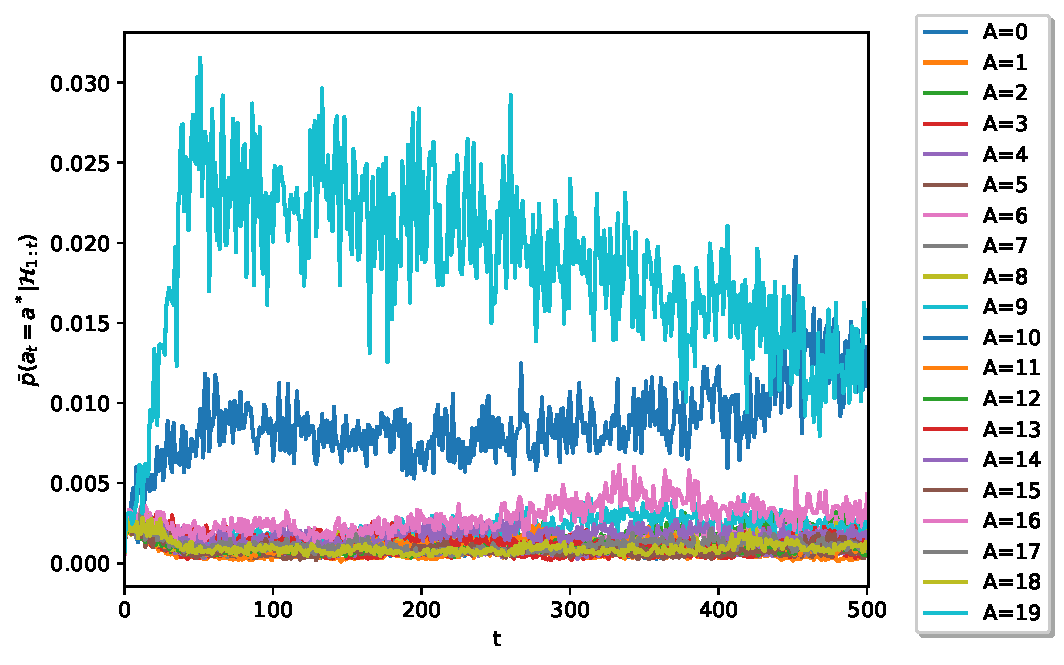
\includegraphics[width=0.85\textwidth]{./fods_figs/yahoo/yahoo_logistic_dynamic}
	\vspace*{-2ex}
	\caption{Empirical probability of playing each bandit arm over time, for SMC-based dynamic logistic Thompson sampling.
		The proposed dynamic bandit policy captures the changing popularity of articles over time.}
	\label{fig:yahoo_logistic_dynamic}
\end{figure}

% Table
%%%%%%%%%%%%%%%%%%%%%%%%
%% Table for yahoo data with logistic bandits
%%%%%%%%%%%%%%%%%%%%%%%%
\begin{table}[!ht]
	\begin{center}
		\resizebox*{\textwidth}{!}{
			\begin{tabular}{*{3}{|c}|}
				\hline
				% Header
				Model \cellcolor[gray]{0.6} & CTR\cellcolor[gray]{0.6} & Normalized CTR\cellcolor[gray]{0.6} \\ \hline
				% table starts
				\cellcolor[gray]{0.8} Logistic rewards, static arms & 0.0670 +/- 0.0088 & 1.6095 +/- 0.2115  \\ \hline
				\cellcolor[gray]{0.8} Logistic rewards, time-evolving arms & 0.0655 +/- 0.0082 & 1.5745 +/- 0.2064 \\ \hline
			\end{tabular}
		}
		\caption{CTR results for SMC-based policies on the news article recommendation dataset.
			The normalized CTR is with respect to a random recommendation baseline.}
		\label{tab:yahoo_logistic_crt}
	\end{center}
	\vspace*{-2ex}
\end{table}

